\documentclass[11pt]{article}

\usepackage[utf8]{inputenc}
\usepackage[T1]{fontenc}
\usepackage{lmodern}
\usepackage{geometry}
\geometry{margin=1in}
\usepackage{amsmath,amssymb,amsfonts,amsthm,mathtools,bm}
\usepackage{microtype}
\usepackage{booktabs}
\usepackage{array}
\usepackage{physics}
\usepackage{tikz}
\usetikzlibrary{arrows.meta,positioning,calc,decorations.pathmorphing,patterns}
\usepackage{hyperref}
\usepackage{enumitem}
\usepackage{authblk}

\hypersetup{
  colorlinks=true,
  linkcolor=blue,
  citecolor=blue,
  urlcolor=blue
}

\newtheorem{theorem}{Theorem}
\newtheorem{proposition}{Proposition}
\newtheorem{lemma}{Lemma}
\newtheorem{definition}{Definition}
\newtheorem{corollary}{Corollary}
\theoremstyle{remark}
\newtheorem{remark}{Remark}

\newcommand{\sinc}{\operatorname{sinc}}
\newcommand{\Sop}{\mathfrak S}
\newcommand{\ShellRes}{\mathcal R}
\newcommand{\Persist}{\mathcal P}
\newcommand{\Access}{\mathcal A}
\newcommand{\Mink}{\mathbb M}

\title{Continuous Operational Shellness of Quantum Field Excitations:\\
Kinematic Mismatch, Persistence, and Finite-Time Detection}
\author{Author Name}
\affil{Independent Research Draft}
\date{\today}

\begin{document}
\maketitle

\begin{abstract}
The exact mass-shell condition is binary: in the metric signature $(-,+,+,+)$, a stable excitation of mass $m$ is on shell when $p^2=-m^2$. This statement is indispensable in scattering theory, but it does not by itself quantify how a finite-duration experiment distinguishes a stable particle, a narrow resonance, a broad continuum excitation, and a strongly off-shell momentum component. We propose a detector-conditioned notion of \emph{operational shellness} that supplements, rather than replaces, the exact mass-shell condition. The construction separates three ingredients that are often conflated: kinematic mismatch from a reference mass shell, temporal persistence of an excitation, and detector accessibility. A detector-frame shell mismatch is derived covariantly from the detector four-velocity. A finite switching window produces a resolution kernel equal to the normalized squared Fourier transform of the switching function; rectangular switching yields the familiar $\sinc^2$ profile, while Gaussian switching yields a Gaussian shell filter. Persistence is defined from a survival amplitude obtained from the excitation's spectral distribution, with exponential decay recovered only as an intermediate-time narrow-width approximation. These ingredients are combined into a normalized operational-shellness functional. We prove boundedness, recover the exact stable-particle limit, derive finite-time shell selection, and obtain protocol-specific necessary and sufficient bounds for direct quasi-particle resolvability. The proposal does not turn perturbative internal lines into detectable particles and does not erase the exact LSZ distinction between stable asymptotic states and non-asymptotic structures. Its purpose is narrower: to provide a mathematically explicit continuum between exact asymptotic particle behavior and detector-inaccessible field excitation, conditional on a stated preparation and measurement protocol.
\end{abstract}

\tableofcontents

\section{Introduction}

The words \emph{on shell}, \emph{off shell}, \emph{real particle}, and \emph{virtual particle} compress several different statements. For a stable species of mass $m$, the equation
\begin{equation}
  p^2=-m^2
  \label{eq:mass-shell}
\end{equation}
is an exact kinematic condition in the metric signature $(-,+,+,+)$. In scattering theory, stable one-particle states appear as isolated poles and define asymptotic in- and out-states through the LSZ construction. Unstable resonances instead correspond to complex poles or broadened spectral structures and are not exact asymptotic one-particle states. Internal propagator momenta in perturbation theory can be off shell, but an internal line is not itself a detector event.

All of these statements remain intact in the present paper. The proposal is not to replace Eq.~\eqref{eq:mass-shell} by a fuzzy equation. Rather, it is to distinguish \emph{exact shell membership} from a second, operational question:
\begin{quote}
Given a prepared excitation, a detector, and a finite interaction time, to what degree does the excitation behave as a persistent and resolvable representative of a chosen particle species?
\end{quote}

This question is naturally continuous. A finite detector has a switching profile, bandwidth, acceptance, coupling, noise floor, and finite observation time. A narrow resonance may produce a sharply reconstructible signal despite not being an asymptotic state. A broad excitation may be visible only as a continuum enhancement. A momentum component displaced from a chosen mass shell may contribute during a finite-time interaction but be rejected in the long-time energy-resolving limit. These are not changes to the exact definition of on shell; they are statements about finite operational resolution.

The central proposal is to separate three quantities:
\begin{enumerate}[label=(\roman*)]
  \item \textbf{kinematic shell resolution}, determined by the mismatch between a four-momentum and a reference mass shell in the detector frame;
  \item \textbf{temporal persistence}, determined by the survival amplitude of the prepared excitation;
  \item \textbf{detector accessibility}, determined by the detector coupling and acceptance.
\end{enumerate}
They may be reported as a three-component \emph{shell profile}, or combined---after a detector protocol is specified---into a scalar operational-shellness functional.

The distinction is important because the K\"all\'en--Lehmann representation alone does not provide a measure of off-shellness. It decomposes a two-point function into positive spectral masses, and each spectral component satisfies its own mass-shell constraint. Off-shellness instead concerns the external momentum at which a propagator or response is evaluated relative to a chosen pole or dispersion relation. The original spectral-only formulation is therefore insufficient for the intended claim. The present construction corrects that conflation.

\paragraph{Limited novelty claim.}
Virtuality, spectral widths, quasiparticle approximations, finite-time detector response, and survival probabilities are all established ideas. The proposed contribution is their explicit separation and recombination into a detector-conditioned functional, together with transparent resolution and measurability bounds. Whether this synthesis is useful must ultimately be judged by applications, not by terminology alone.

\section{What is exact, what is continuous, and what is measured}

\subsection{Exact shell membership}

For a stable relativistic species with mass $m$, the future mass shell is
\begin{equation}
  \mathcal H_m^+
  =\left\{p\in\Mink^4:\ p^2=-m^2,\ p^0>0\right\}.
\end{equation}
Membership in $\mathcal H_m^+$ is binary. A four-momentum either satisfies the equation or it does not. This paper does not modify that fact.

\subsection{Spectral stability and resonance width}

For a scalar field, the vacuum two-point function has the K\"all\'en--Lehmann form
\begin{equation}
  G_F(p)
  =\int_0^\infty \dd s\,\rho(s)
  \frac{-i}{p^2+s-i\epsilon},
  \label{eq:KL}
\end{equation}
with $\rho(s)\ge 0$ under the standard positivity assumptions. A stable one-particle state contributes
\begin{equation}
  \rho(s)=Z\,\delta(s-m^2)+\rho_{\mathrm{cont}}(s),
  \qquad Z>0.
  \label{eq:stable-pole-density}
\end{equation}
An unstable resonance does not contribute a normalizable asymptotic delta function. Near a narrow resonance, one often uses the approximation
\begin{equation}
  \rho_R(s)
  \approx \frac{1}{\pi}
  \frac{M\Gamma}{(s-M^2)^2+M^2\Gamma^2},
  \label{eq:breit-wigner}
\end{equation}
within a restricted range where threshold effects and energy dependence of the self-energy can be neglected.

Equation~\eqref{eq:KL} is a spectral decomposition, not a probability distribution over ``how virtual'' a particle is. The integration variable $s$ labels invariant masses of physical spectral support. The momentum $p$ at which $G_F(p)$ is evaluated can still be displaced from every singular structure in the integral.

\subsection{Detector response}

A minimal operational model is a localized two-level probe coupled to a field operator $\mathcal O$. Along a detector worldline $x(\tau)$, let
\begin{equation}
  H_I(\tau)
  =\lambda\,\chi_T(\tau)\,\hat m(\tau)\,\mathcal O(x(\tau)),
  \label{eq:UDW-interaction}
\end{equation}
where $\chi_T$ is a switching function, $\lambda$ is a weak coupling, and $\hat m$ is the detector monopole operator. To leading nontrivial order, the excitation probability is
\begin{align}
  P_{g\to e}
  ={}&\lambda^2
  \left|\matrixel{e}{\hat m(0)}{g}\right|^2
  \int \dd\tau\,\dd\tau'\,
  \chi_T(\tau)\chi_T(\tau')
  e^{-i\Omega_D(\tau-\tau')}
  \nonumber\\
  &\hspace{2cm}\times
  W_{\mathcal O}(x(\tau),x(\tau')),
  \label{eq:detector-response}
\end{align}
where $\Omega_D$ is the detector gap and $W_{\mathcal O}$ is a Wightman correlation function. Equation~\eqref{eq:detector-response} makes the operational point precise: a detector measures field correlations filtered by its trajectory, switching, gap, and coupling. It does not observe an individual perturbative internal line.

\section{Detector-frame shell mismatch}

Let $u^\mu$ be the future-directed four-velocity of an inertial detector, normalized by
\begin{equation}
  u^2=-1.
\end{equation}
For any future-directed four-momentum $p^\mu$, define the detector-frame energy
\begin{equation}
  \omega_u(p)=-u\cdot p
  \label{eq:detector-energy}
\end{equation}
and the spatial projector
\begin{equation}
  h^{\mu\nu}=\eta^{\mu\nu}+u^\mu u^\nu.
\end{equation}
The spatial momentum magnitude measured by the detector is
\begin{equation}
  k_u^2(p)=h_{\mu\nu}p^\mu p^\nu
  =p^2+(u\cdot p)^2.
\end{equation}
For a reference species of mass $m$, the on-shell energy associated with the same detector-frame spatial momentum is
\begin{equation}
  \Omega_m(p;u)=\sqrt{m^2+k_u^2(p)}.
  \label{eq:on-shell-energy}
\end{equation}

\begin{definition}[Detector-frame shell mismatch]
The shell mismatch of $p$ relative to mass $m$ and detector velocity $u$ is
\begin{equation}
  \delta_u(p;m)
  =\omega_u(p)-\Omega_m(p;u).
  \label{eq:shell-mismatch}
\end{equation}
\end{definition}

This quantity has dimensions of energy and is directly matched to finite-time energy resolution. It is observer-dependent in exactly the same controlled sense that detector energy is observer-dependent. The underlying mass-shell equation remains Lorentz invariant.

\begin{proposition}[Equivalence with the exact mass shell]
For future-directed $p$ and $m\ge 0$,
\begin{equation}
  \delta_u(p;m)=0
  \quad\Longleftrightarrow\quad
  p^2=-m^2.
  \label{eq:equivalence}
\end{equation}
Moreover,
\begin{equation}
  p^2+m^2
  =-\delta_u(p;m)
  \left[\omega_u(p)+\Omega_m(p;u)\right].
  \label{eq:virtuality-mismatch-relation}
\end{equation}
\end{proposition}

\begin{proof}
Using $p^2=-\omega_u^2+k_u^2$ and
$\Omega_m^2=m^2+k_u^2$,
\begin{align}
  p^2+m^2
  &=\Omega_m^2-\omega_u^2\\
  &=(\Omega_m-\omega_u)(\Omega_m+\omega_u)\\
  &=-\delta_u(\Omega_m+\omega_u).
\end{align}
For future-directed $p$, both energies are nonnegative, and the second factor is positive except for the trivial massless zero-momentum case. Thus $p^2=-m^2$ if and only if $\delta_u=0$.
\end{proof}

Equation~\eqref{eq:virtuality-mismatch-relation} is the desired bridge between the invariant equation $p^2=-m^2$ and the detector's finite-time frequency mismatch. It also shows why $p^2+m^2$ alone is not the most convenient operational variable: a detector resolves frequencies, not mass-squared directly.

\section{Finite-time shell resolution}

A detector interacting for finite proper time cannot impose an exact frequency delta function. Let $\chi_T\in L^1(\mathbb R)$ be a nonnegative switching profile with
\begin{equation}
  0<\int_{-\infty}^{\infty}\chi_T(\tau)\,\dd\tau<\infty.
\end{equation}
Define its Fourier transform by
\begin{equation}
  \widehat\chi_T(\nu)
  =\int_{-\infty}^{\infty}\chi_T(\tau)e^{i\nu\tau}\,\dd\tau.
\end{equation}

\begin{definition}[Finite-time shell-resolution kernel]
The normalized shell-resolution kernel is
\begin{equation}
  \ShellRes_{\chi,T}(p;m,u)
  =\frac{
  \left|\widehat\chi_T\!\left(\delta_u(p;m)\right)\right|^2
  }{
  \left|\widehat\chi_T(0)\right|^2
  }.
  \label{eq:resolution-kernel}
\end{equation}
\end{definition}

\begin{theorem}[Resolution-kernel bounds]
If $\chi_T\ge0$ almost everywhere, then
\begin{equation}
  0\le \ShellRes_{\chi,T}(p;m,u)\le1,
\end{equation}
and $\ShellRes_{\chi,T}=1$ whenever $p$ is exactly on the reference shell.
\end{theorem}

\begin{proof}
Nonnegativity is immediate. By the triangle inequality,
\begin{equation}
  \left|\widehat\chi_T(\nu)\right|
  \le \int \chi_T(\tau)\,\dd\tau
  =\widehat\chi_T(0).
\end{equation}
Squaring and normalizing gives the upper bound. If $\delta_u=0$, numerator and denominator coincide.
\end{proof}

\subsection{Rectangular switching}

For a rectangular window of duration $T$,
\begin{equation}
  \chi_T(\tau)=\mathbf 1_{[-T/2,T/2]}(\tau),
\end{equation}
we obtain
\begin{equation}
  \ShellRes_{\mathrm{rect},T}(p;m,u)
  =\sinc^2\!\left(
  \frac{T\,\delta_u(p;m)}{2}
  \right),
  \qquad
  \sinc x=\frac{\sin x}{x}.
  \label{eq:sinc-kernel}
\end{equation}
The first zeros occur at
\begin{equation}
  |\delta_u|=\frac{2\pi}{T}.
\end{equation}
Thus longer interaction time narrows the accepted shell neighborhood.

\subsection{Gaussian switching}

For
\begin{equation}
  \chi_T(\tau)=e^{-\tau^2/(2T^2)},
\end{equation}
the normalized kernel is
\begin{equation}
  \ShellRes_{\mathrm{G},T}(p;m,u)
  =e^{-T^2\delta_u(p;m)^2}.
  \label{eq:gaussian-kernel}
\end{equation}
The Gaussian window is analytically convenient because it has no side lobes.

\begin{remark}[What finite time does not imply]
A nonzero value of $\ShellRes_{\chi,T}$ away from the shell does not convert an off-shell propagator component into an asymptotic particle. It states only that a finite switching window cannot perfectly discriminate the corresponding frequency mismatch.
\end{remark}

\section{Temporal persistence from spectral support}

A lifetime parameter should not be inserted without specifying what persists. Let $\ket{\Psi}$ be a normalized prepared state or projected excitation. Its survival amplitude is
\begin{equation}
  a_\Psi(T)
  =\mel{\Psi}{e^{-iHT}}{\Psi},
  \label{eq:survival-amplitude}
\end{equation}
and its survival probability is
\begin{equation}
  \Persist_\Psi(T)=|a_\Psi(T)|^2.
  \label{eq:survival-probability}
\end{equation}
By the spectral theorem, there exists a normalized positive energy distribution $\varpi_\Psi(E)$ such that
\begin{equation}
  a_\Psi(T)
  =\int_{E_{\min}}^\infty
  \varpi_\Psi(E)e^{-iET}\,\dd E,
  \qquad
  \int_{E_{\min}}^\infty\varpi_\Psi(E)\,\dd E=1.
  \label{eq:fock-krylov}
\end{equation}

\begin{proposition}[Persistence bounds]
For every normalized $\ket{\Psi}$,
\begin{equation}
  0\le\Persist_\Psi(T)\le1,
  \qquad
  \Persist_\Psi(0)=1.
\end{equation}
\end{proposition}

\begin{proof}
Unitarity gives
$|\mel{\Psi}{e^{-iHT}}{\Psi}|\le
\|\Psi\|\,\|e^{-iHT}\Psi\|=1$.
\end{proof}

For an isolated stable energy eigenstate, $\Persist_\Psi(T)=1$. For a narrow unstable resonance over its approximately exponential regime,
\begin{equation}
  \Persist_\Psi(T)\approx e^{-\Gamma T}.
  \label{eq:exponential-approx}
\end{equation}
However, exact quantum survival is generally nonexponential at sufficiently short and long times. For this reason, the primary definition is Eq.~\eqref{eq:survival-probability}; Eq.~\eqref{eq:exponential-approx} is a controlled model approximation, not a universal law.

\section{Detector accessibility}

The shell-resolution kernel and survival probability do not yet say whether the detector couples to the excitation. Introduce a measurable acceptance function
\begin{equation}
  0\le \Access_D(p)\le1,
  \label{eq:acceptance}
\end{equation}
which may encode geometry, polarization, charge sensitivity, threshold, efficiency, and normalized matrix-element weight. In a detailed detector theory, $\Access_D$ must be derived from a response such as Eq.~\eqref{eq:detector-response}. In a phenomenological model, it may be estimated from calibration data.

Let $w_\Psi(p)\ge0$ be a normalized momentum-space weight for the prepared excitation,
\begin{equation}
  \int \dd\Pi(p)\,w_\Psi(p)=1,
  \label{eq:packet-normalization}
\end{equation}
where $\dd\Pi(p)$ denotes the protocol-appropriate momentum measure. The framework does not require $w_\Psi$ to be a free one-particle distribution; it may be constructed from a wave packet, a positive-frequency spectral function, or a reconstructed event ensemble.

\section{Operational shellness}

\begin{definition}[Shell profile]
For a specified excitation, detector, duration, reference mass, and detector velocity, define
\begin{align}
  Q_{\mathrm{shell}}
  &=\frac{\int \dd\Pi(p)\,w_\Psi(p)\Access_D(p)
  \ShellRes_{\chi,T}(p;m,u)}
  {\int \dd\Pi(p)\,w_\Psi(p)\Access_D(p)},
  \\
  Q_{\mathrm{pers}}
  &=\Persist_\Psi(T),
  \\
  Q_{\mathrm{acc}}
  &=\int \dd\Pi(p)\,w_\Psi(p)\Access_D(p),
\end{align}
provided the first denominator is nonzero. The ordered triple
\begin{equation}
  \mathbf Q_{D,T}[\Psi;m,u]
  =\left(Q_{\mathrm{shell}},Q_{\mathrm{pers}},Q_{\mathrm{acc}}\right)
  \label{eq:shell-profile}
\end{equation}
is the \emph{shell profile}.
\end{definition}

The profile is more informative than one number: an excitation may be close to shell but short-lived, persistent but outside detector acceptance, or detectable without matching the chosen particle species.

\begin{definition}[Conditional shell-persistence score]
When a scalar summary conditional on detector overlap is useful, define
\begin{equation}
  \Sop^{\mathrm{cond}}_{D,T}[\Psi;m,u]
  =\frac{
  \int \dd\Pi(p)\,w_\Psi(p)\Access_D(p)
  \ShellRes_{\chi,T}(p;m,u)
  \Persist_\Psi(T\mid p)
  }{
  \int \dd\Pi(p)\,w_\Psi(p)\Access_D(p)
  },
  \label{eq:conditional-shellness}
\end{equation}
provided the denominator is finite and nonzero. Here
$\Persist_\Psi(T\mid p)\in[0,1]$ is a momentum-resolved survival factor when such a decomposition is meaningful. If persistence is not momentum-resolved, one sets
$\Persist_\Psi(T\mid p)=\Persist_\Psi(T)$.
\end{definition}

\begin{definition}[Operational detectability score]
Because $w_\Psi$ is normalized, the detector-inclusive scalar is
\begin{equation}
  \Sop^{\mathrm{op}}_{D,T}[\Psi;m,u]
  =
  \int \dd\Pi(p)\,w_\Psi(p)\Access_D(p)
  \ShellRes_{\chi,T}(p;m,u)
  \Persist_\Psi(T\mid p).
  \label{eq:operational-shellness}
\end{equation}
It satisfies
\begin{equation}
  \Sop^{\mathrm{op}}_{D,T}
  =Q_{\mathrm{acc}}\,
  \Sop^{\mathrm{cond}}_{D,T}.
  \label{eq:op-cond-relation}
\end{equation}
Thus detector inefficiency is not silently normalized away.
\end{definition}

\begin{theorem}[Boundedness]
Under the assumptions above,
\begin{equation}
  0\le \Sop^{\mathrm{cond}}_{D,T}\le1,
  \qquad
  0\le \Sop^{\mathrm{op}}_{D,T}\le1.
\end{equation}
\end{theorem}

\begin{proof}
Every factor is nonnegative and bounded by unity. For the conditional score, the numerator is bounded above by its denominator. For the operational score, the integrand is bounded above by $w_\Psi$, whose integral is one.
\end{proof}

\begin{proposition}[Exact stable-particle limit]
Suppose $w_\Psi$ has support entirely on $\mathcal H_m^+$ and the excitation is stable, so that $\Persist_\Psi(T\mid p)=1$. Then
\begin{equation}
  \Sop^{\mathrm{cond}}_{D,T}=1,
  \qquad
  \Sop^{\mathrm{op}}_{D,T}=Q_{\mathrm{acc}}
\end{equation}
for every $T$ and every nonnegative switching profile. In particular, an ideal detector with unit acceptance has $\Sop^{\mathrm{op}}_{D,T}=1$.
\end{proposition}

\begin{proof}
On the support of $w_\Psi$, Eq.~\eqref{eq:equivalence} gives $\delta_u=0$, hence $\ShellRes_{\chi,T}=1$. Substitution into Eqs.~\eqref{eq:conditional-shellness} and \eqref{eq:operational-shellness} gives the result.
\end{proof}

\begin{proposition}[Finite-time shell selection]
For rectangular switching and a single momentum component,
\begin{equation}
  \Sop^{\mathrm{op}}(T)
  =\Access_D(p)\,
  \Persist_\Psi(T\mid p)\,
  \sinc^2\!\left(\frac{\delta_uT}{2}\right).
  \label{eq:single-mode-rect}
\end{equation}
For fixed $\delta_u\neq0$, the shell-resolution factor tends to zero as $T\to\infty$; for $\delta_u=0$, it remains unity.
\end{proposition}

This is the sense in which the exact shell condition emerges from arbitrarily long frequency discrimination. It is not a statement that finite-time dynamics violates energy conservation; it is a statement about the width of the measurement filter.

\section{Protocol-specific measurability bounds}

There is no detector-independent boundary between ``measurable'' and ``unmeasurable.'' A bound requires at least:
\begin{enumerate}[label=(\roman*)]
  \item a detector protocol;
  \item a minimum accepted score $q\in(0,1)$;
  \item a minimum interaction or integration time $T_{\min}$;
  \item a detector accessibility $\eta=\Access_D(p)$ for the mode of interest.
\end{enumerate}

Consider a single approximately exponential mode observed with Gaussian switching. Combining Eqs.~\eqref{eq:gaussian-kernel} and \eqref{eq:exponential-approx} gives
\begin{equation}
  \Sop^{\mathrm{op}}_{\mathrm G}(T)
  =\eta\,e^{-\Gamma T-T^2\delta_u^2}.
  \label{eq:gaussian-score}
\end{equation}

\begin{theorem}[Exact threshold criterion in the Gaussian model]
Let $0<q\le\eta\le1$. The condition
\begin{equation}
  \Sop^{\mathrm{op}}_{\mathrm G}(T)\ge q
\end{equation}
is equivalent to
\begin{equation}
  \Gamma T+\delta_u^2T^2
  \le\ln\!\left(\frac{\eta}{q}\right).
  \label{eq:threshold-bound}
\end{equation}
If the detector requires $T\ge T_{\min}$, then there exists an admissible interaction time if and only if
\begin{equation}
  \Gamma T_{\min}+\delta_u^2T_{\min}^2
  \le\ln\!\left(\frac{\eta}{q}\right).
  \label{eq:existence-bound}
\end{equation}
\end{theorem}

\begin{proof}
Taking the logarithm of Eq.~\eqref{eq:gaussian-score} yields Eq.~\eqref{eq:threshold-bound}. The left-hand side is nondecreasing for $T\ge0$, $\Gamma\ge0$, so among all $T\ge T_{\min}$ it is minimized at $T_{\min}$.
\end{proof}

Equation~\eqref{eq:existence-bound} is a concrete answer to the question ``how long must an excitation persist to be directly resolvable?'' within the stated model. The answer is not a universal lifetime. It is a joint constraint on lifetime, shell mismatch, detector coupling, acceptance threshold, and required integration time.

For an exactly shell-matched mode, $\delta_u=0$, Eq.~\eqref{eq:existence-bound} reduces to
\begin{equation}
  \Gamma T_{\min}
  \le\ln\!\left(\frac{\eta}{q}\right).
  \label{eq:lifetime-only-bound}
\end{equation}
Equivalently, with $\tau=\Gamma^{-1}$,
\begin{equation}
  \tau
  \ge
  \frac{T_{\min}}{\ln(\eta/q)}.
  \label{eq:lifetime-lower-bound}
\end{equation}
For a perfectly persistent mode, $\Gamma=0$, the shell mismatch must satisfy
\begin{equation}
  |\delta_u|
  \le
  \frac{1}{T_{\min}}
  \sqrt{\ln\!\left(\frac{\eta}{q}\right)}.
  \label{eq:mismatch-bound}
\end{equation}

\begin{remark}[Direct and indirect detection]
Equations~\eqref{eq:existence-bound}--\eqref{eq:mismatch-bound} concern direct quasi-particle resolution by the specified finite-time filter. Short-lived resonances can still be measured indirectly through decay products and invariant-mass reconstruction even when they cannot propagate to a detector as persistent one-particle states. ``Measurable'' must therefore always name the measurement channel.
\end{remark}

\section{Toy model: a stable pole opening into a resonance}

Consider two real scalar fields with interaction
\begin{equation}
  \mathcal L
  =-\frac12\partial_\mu\Phi\partial^\mu\Phi
   -\frac12M_0^2\Phi^2
   -\frac12\partial_\mu\chi\partial^\mu\chi
   -\frac12m^2\chi^2
   -g\Phi\chi^2.
  \label{eq:toy-lagrangian}
\end{equation}
The dressed $\Phi$ propagator may be written schematically as
\begin{equation}
  G_\Phi(p)
  =\frac{-i}{p^2+M_0^2+\Sigma(p^2)-i\epsilon}.
  \label{eq:dressed-propagator}
\end{equation}
Below the two-$\chi$ threshold, a pole may lie on the physical real axis and represent a stable state. Above threshold, the self-energy acquires an imaginary part. A narrow resonance pole appears on an unphysical sheet near
\begin{equation}
  p^2\approx -M^2+iM\Gamma.
  \label{eq:complex-pole}
\end{equation}
In the resonance regime, the spectral enhancement may be approximated by Eq.~\eqref{eq:breit-wigner}, and the intermediate-time survival probability is approximately $e^{-\Gamma T}$.

For a packet concentrated near one detector-frame momentum, Gaussian switching gives
\begin{equation}
  \Sop^{\mathrm{op}}_{\mathrm G}(T)
  \approx\eta\,
  \exp\!\left[-\Gamma T
  -T^2\left(
  \omega_u-\sqrt{M^2+k_u^2}
  \right)^2\right].
  \label{eq:toy-score}
\end{equation}
The two suppressions have distinct meanings. The term $\Gamma T$ penalizes failure to persist. The term $T^2\delta_u^2$ penalizes mismatch from the chosen dispersion relation at the detector's frequency resolution.

\begin{figure}[t]
\centering
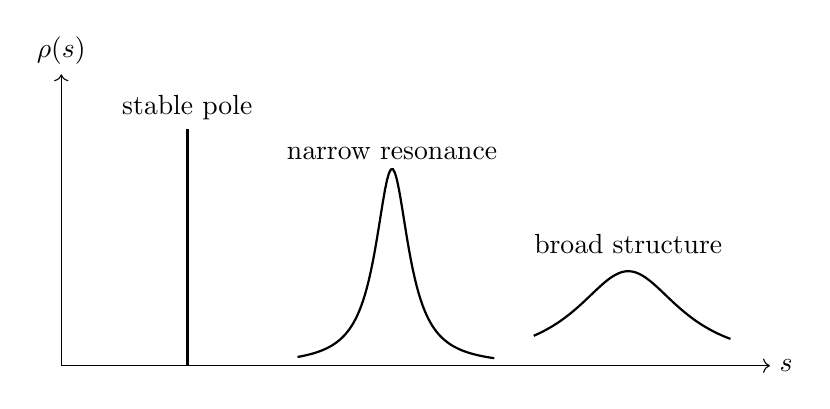
\begin{tikzpicture}[x=1.0cm,y=1.0cm]
  \draw[->] (0,0) -- (9,0) node[right] {$s$};
  \draw[->] (0,0) -- (0,3.7) node[above] {$\rho(s)$};
  \draw[very thick] (1.6,0) -- (1.6,3.0);
  \node[above] at (1.6,3.0) {stable pole};
  \draw[thick,domain=3.0:5.5,samples=100]
  plot (\x,{2.5/(1+15*(\x-4.2)*(\x-4.2))});
  \node[above] at (4.2,2.5) {narrow resonance};
  \draw[thick,domain=6.0:8.5,samples=100]
  plot (\x,{1.2/(1+1.5*(\x-7.2)*(\x-7.2))});
  \node[above] at (7.2,1.3) {broad structure};
\end{tikzpicture}
\caption{Spectral stability is continuous through widths and continuum structure, whereas exact stable-particle pole membership remains discrete. Operational shellness combines this spectral persistence with finite-time shell resolution and detector acceptance.}
\label{fig:spectral-structures}
\end{figure}

\section{Relation to virtual particles}

The framework must not be read as an ontology of virtual particles. An internal line in a Feynman diagram is an element of a perturbative representation of an amplitude. Its momentum can be off shell, and different gauges, field variables, or rearrangements of perturbation theory can alter the intermediate description while leaving observables invariant.

Operational shellness applies to a specified excitation weight and detector response. It can quantify how strongly a prepared or reconstructed field excitation resembles a persistent excitation of a reference species. It does not assign a detector-independent existence score to every internal propagator line.

The appropriate reinterpretation is therefore:
\begin{quote}
The exact real/virtual distinction used in scattering theory should not be replaced by a continuum. Instead, finite experimental particle-likeness can be represented continuously after exact kinematic, spectral, and detector notions have been separated.
\end{quote}

\section{Comparison with the original spectral-only functional}

A spectral-only proposal of the form
\begin{equation}
  \frac{\int \dd s\,\rho(s)K_D(s)e^{-T\Gamma(s)}}
  {\int \dd s\,\rho(s)K_D(s)}
  \label{eq:old-functional}
\end{equation}
contains a useful intuition but cannot serve as a general measure of shellness.

First, $s$ is a spectral mass variable, not the off-shell momentum mismatch of a propagator. Second, $e^{-T\Gamma}$ assumes a purely exponential survival law and does not identify the prepared state whose survival is being measured. Third, a kernel in $s$ alone omits detector-frame frequency mismatch and switching-time resolution. Fourth, monotonic decrease in $T$ is not a universal theorem for exact quantum survival probabilities, which may display short-time quadratic behavior, late-time power-law tails, or revivals.

Equations~\eqref{eq:conditional-shellness} and \eqref{eq:operational-shellness} retain the useful detector weighting while correcting these limitations. The old functional is recovered only as a restricted approximation when:
\begin{enumerate}[label=(\roman*)]
  \item the excitation is diagonalized by a spectral mass label $s$;
  \item the detector kernel depends only on $s$;
  \item the shell-resolution factor is taken as unity over the selected band;
  \item each component has an approximately exponential survival law.
\end{enumerate}
Thus the previous expression should be treated as a special coarse-grained persistence average, not as the foundational definition.

\section{Interpretation and limits}

The proposed framework supports four distinct statements.

\paragraph{Exact on shell.}
A stable future-directed momentum satisfies $p^2=-m^2$. This is binary and detector-independent.

\paragraph{Approximately shell matched.}
A finite detector accepts a neighborhood of the exact shell determined by the Fourier width of its switching profile. This is continuous and detector-dependent.

\paragraph{Persistent.}
A prepared excitation has a survival probability. Stable states persist exactly; narrow resonances persist approximately over intermediate times; broad structures generally do not admit a long-lived one-particle interpretation.

\paragraph{Accessible.}
A detector responds only through allowed couplings, thresholds, geometry, and readout. Accessibility is not implied by shell matching or persistence alone.

These four statements should not be collapsed into the single everyday word ``real.'' The framework makes the compression explicit while retaining the standard QFT categories underneath.

Several limitations remain. The present paper treats scalar kinematics and a simple detector frame. Spin, gauge constraints, confinement, medium-dependent dispersion relations, noninertial trajectories, and fully interacting detector models require separate treatment. In gauge theories, a proposed excitation weight must be built from gauge-invariant observables or a carefully fixed operational protocol. In confined theories, quark and gluon propagator virtualities cannot be interpreted as direct particle observability scores. Finally, the scalar score in Eq.~\eqref{eq:operational-shellness} is not unique; the shell profile in Eq.~\eqref{eq:shell-profile} should be retained whenever different tradeoffs matter.

\section{Conclusion}

The on-shell equation $p^2=-m^2$ is exact and should remain exact. What is incomplete is using that equation alone as the full language of experimentally realized particle behavior. A finite experiment simultaneously probes shell mismatch, persistence, and detector accessibility.

We derived a detector-frame energy mismatch equivalent to the invariant mass-shell equation, showed how a finite switching function converts this mismatch into a continuous resolution kernel, defined persistence from a survival amplitude rather than an assumed width, and combined these ingredients into a normalized operational-shellness functional. For a Gaussian finite-time protocol and an approximately exponential resonance, the direct resolvability condition is
\begin{equation}
  \Gamma T_{\min}+\delta_u^2T_{\min}^2
  \le\ln\!\left(\frac{\eta}{q}\right).
\end{equation}
This is not a universal boundary between real and virtual particles. It is a protocol-specific bound describing when a prepared excitation can be resolved as a persistent representative of a chosen particle species.

The resulting perspective is therefore precise but conservative:
\begin{quote}
Exact shell membership is binary; operational particle-likeness is continuous.
\end{quote}

\begin{thebibliography}{99}

\bibitem{Kallen1952}
G.~K\"all\'en,
``On the definition of the renormalization constants in quantum electrodynamics,''
\textit{Helvetica Physica Acta} \textbf{25}, 417--434 (1952).

\bibitem{Lehmann1954}
H.~Lehmann,
``\"Uber Eigenschaften von Ausbreitungsfunktionen und Renormierungskonstanten quantisierter Felder,''
\textit{Nuovo Cimento} \textbf{11}, 342--357 (1954).

\bibitem{LSZ1955}
H.~Lehmann, K.~Symanzik, and W.~Zimmermann,
``Zur Formulierung quantisierter Feldtheorien,''
\textit{Nuovo Cimento} \textbf{1}, 205--225 (1955).

\bibitem{Ruelle1962}
D.~Ruelle,
``On the asymptotic condition in quantum field theory,''
\textit{Helvetica Physica Acta} \textbf{35}, 147--163 (1962).

\bibitem{PeskinSchroeder}
M.~E.~Peskin and D.~V.~Schroeder,
\textit{An Introduction to Quantum Field Theory},
Addison--Wesley (1995).

\bibitem{WeinbergQFT}
S.~Weinberg,
\textit{The Quantum Theory of Fields, Vol.~I},
Cambridge University Press (1995).

\bibitem{Haag}
R.~Haag,
\textit{Local Quantum Physics}, 2nd ed.,
Springer (1996).

\bibitem{Unruh1976}
W.~G.~Unruh,
``Notes on black-hole evaporation,''
\textit{Physical Review D} \textbf{14}, 870--892 (1976).

\bibitem{DeWitt1979}
B.~S.~DeWitt,
``Quantum gravity: the new synthesis,''
in \textit{General Relativity: An Einstein Centenary Survey},
Cambridge University Press (1979).

\bibitem{Garay2016}
L.~J.~Garay, E.~Mart\'in-Mart\'inez, and J.~de Ram\'on,
``Thermalization of particle detectors: The Unruh effect and its reverse,''
\textit{Physical Review D} \textbf{94}, 104048 (2016),
arXiv:1607.05287.

\bibitem{AartsBerges2001}
G.~Aarts and J.~Berges,
``Nonequilibrium time evolution of the spectral function in quantum field theory,''
\textit{Physical Review D} \textbf{64}, 105010 (2001),
arXiv:hep-ph/0103049.

\bibitem{Berges2004}
J.~Berges,
``Introduction to nonequilibrium quantum field theory,''
\textit{AIP Conference Proceedings} \textbf{739}, 3--62 (2004),
arXiv:hep-ph/0409233.

\bibitem{Beneke2015}
M.~Beneke,
``Unstable-particle effective field theory,''
\textit{Nuclear and Particle Physics Proceedings} \textbf{261--262}, 218--231 (2015),
arXiv:1501.07370.

\bibitem{Aoki2023}
K.~Aoki,
``Unitarity and unstable-particle scattering amplitudes,''
\textit{Physical Review D} \textbf{107}, 065017 (2023),
arXiv:2212.05670.

\bibitem{RamirezKelkar2021}
D.~F.~Ram\'irez Jim\'enez and N.~G.~Kelkar,
``Formal aspects of quantum decay,''
\textit{Physical Review A} \textbf{104}, 022214 (2021),
arXiv:2108.10957.

\bibitem{Luscher1991}
M.~L\"uscher,
``Signatures of unstable particles in finite volume,''
\textit{Nuclear Physics B} \textbf{364}, 237--254 (1991).

\end{thebibliography}

\end{document}
